\section{Material models and results}
\label{sec:results}

In this section, we present specific material models and parameter estimation results using our Bayesian inference framework with summary functions. We show four different material models: bumpy microfacet surface, brushed metal, metallic paint with flakes, and scattering medium. We include a mix of synthetic and real results.

Except for the scattering example, the camera and light are co-located; this matches a mobile phone camera fairly closely, and simplifies some BRDF formulations, because the incoming, outgoing, and half vector are all identical in this case.

All photographs are taken with an iPhone 7 in the raw format and saved as a linear DNG file. We use the Adobe Lightroom mobile app in manual mode for capture, adjusting exposure down so that the areas overexposed from flash are reduced. For some materials, overexposure is unavoidable; we simply let overly bright areas clamp, and apply the same clamping to our forward simulation, instead of working with multi-exposure HDR images, which are highly inconvenient for hand-held mobile phone photography.

In our examples, we assume the distance between camera and sample is known; this is not difficult to measure or estimate. If this estimate is off by a constant, the resulting material scale will be off by the same constant ratio, because the configuration is scale-invariant. The knowledge of the camera field of view lets us compute the physical scale of the resulting pixels. Note that we use real-world units (centimeters) in all forward simulations; this ensures that the resulting materials have physical proportions.

All our material models are implemented using \torch, using array-level operations; this automatically provides GPU acceleration and computes derivatives through backpropagation, and lets us express fairly complex operations, including microfacet BRDF evaluation, binning and fast Fourier transforms. We use a resolution of $512 \times 512$ for all simulated images except in the metallic paint model ($256 \times 256$). The GPU we use is an Nvidia GTX 1080.

\begin{table}[t]
\caption{Performance statistics for our HMC-based posterior sampling processes. Sample count: 50k.\label{fig:performance}}
\begin{tabular}{l|c|c|c}
	%\hline
	Material &Tot. eval & Time & eval/sec \\
	Bumpy surface    &100k & 23 mins & 72 \\
	Brushed Metal    &114k & 30 mins & 63 \\
	Metallic flakes  &113k & 24 mins & 78 \\
	Scatter w/o surf.&100k & 600 mins & 2.7 \\
	Scatter with surf.& 103k & 820 mins & 2.1
\end{tabular}
\end{table}

\subsection{Bumpy microfacet surface}

This material models an opaque dielectric surface with an isotropic noise heightfield, common in wall paints, plastics, and more. We use a standard microfacet BRDF with the GGX normal distribution \cite{Walter2007}, in combination with a normal map computed from an explicitly constructed heightfield. We assume the Fresnel reflectance at normal incidence can be computed from a known index of refraction; a value of 1.5 tends to be a good estimate for plastics. We assume an unknown roughness $r$ (GGX parameter $\alpha=r^2$) and a Lambertian diffuse term with unknown albedo $\rho$.

The bumpy heightfield is constructed using an inverse Fourier process, similar to \cite{Wang2011}. This is based on choosing a power spectrum in the continuous Fourier domain, discretizing it onto a grid of complex numbers, randomly choosing the phase of each texel on the grid (while keeping the chosen amplitude), and finally taking an inverse fast Fourier transform, the real component of which becomes the resulting heightfield. The normal map can be computed from the heightfield (finite differences work well).

We follow Wang et al. in choosing the power spectrum to be a Gaussian, with standard deviation $\fsigma$ and a scaling coefficient $\fscale$. The units in the continuous Fourier domain will be cm$^{-1}$, therefore, these will also be the units of the $\fsigma$ parameter, and the discretization needs to consider this. Note an advantage of using real-world units independent of discretization: once the parameters $\fsigma$ and $\fscale$ are estimated, this material's textures can be realized at any resolution; there is no limitation to use the resolution used for parameter estimation also in final rendering.

We additionally model the light intensity as an unknown RGB triple $\light$, thus we do not require any tedious calibration procedures. Finally, we observed on this example that the vignetting from the iPhone camera has an impact on the results. While we could post-process the images to counter the effect, we find it easier and more appropriate within our framework to simply model the vignetting as a broad Gaussian, whose standard deviation becomes yet another parameter $\sigma_v$. The full parameter vector of this model is therefore
\[
\btheta = (\rho, r, \fsigma, \fscale, \light, \sigma_v),
\]
while the random latent vector $\bz$ is used to choose the phase randomization above. This model is fairly similar to Wang et al. \shortcite{Wang2011}, though using the GGX instead of Beckmann microfacet distribution. The main practical difference from the capture setup in that paper is that we use a point light, instead of step-edge illumination.

Next, we show several synthetic examples, each meant to illustrate the behavior of a specific summary function. The target image we are matching in these examples is shown in Figure \ref{fig:bump-synth-gt} (left). The simplest summary function we applied to this case is \emph{concentric means}: this function simply puts the image pixels into 64 bins based on their distance from the image center; the pixels further than a threshold are discarded. Then a mean is computed over each bin, in 3 RGB channels. The results with this summary function can be seen in Figure \ref{fig:bump-synth0}.

Clearly, a more powerful summary function is needed here. One idea is to combine concentric means with \emph{concentric standard deviations}. The result with this summary function is significantly improved, and can be seen in Figure \ref{fig:bump-synth1}. Yet another idea is to use a 2D Fourier transform of the image, and compute concentric means of that, which is an efficient way to summarize the frequency content of the image. We find this summary function behaves comparably and in some cases better than the previous ones; the result can be seen in Figure \ref{fig:bump-synth2}.

Finally, we show a result using the FFT summary function on a real example; the target photograph of a red wall paint, together with our match, can be seen in Figure \ref{fig:bump-real-gt}. The result of the posterior sampling can be seen in Figure \ref{fig:bump-real}. In summary, we believe our solution is comparable in quality to Wang et al. \shortcite{Wang2011}, but compared to their heavily specialized solution for this material model, our framework is much more general, and a flash photograph is an even more convenient capture method than their step-edge illumination.


\begin{figure}[t]
	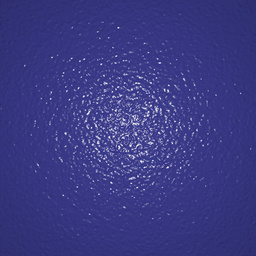
\includegraphics[width=0.49\columnwidth]{results/bump/syn_comp/bump02rd1.png}
	\includegraphics[width=0.49\columnwidth]{results/bump/syn2/bestfit.png}
	\caption{Synthetic bumpy surface example. Left: Target synthetic image (reference). Right: Best match found through our method using the FFT-based summary function.}
	\label{fig:bump-synth-gt}
\end{figure}

\begin{figure}[t]
	\includegraphics[width=\columnwidth]{results/bump/syn0/posterior.pdf}
	\addtolength{\tabcolsep}{-3.5pt}
	\begin{tabular}{ccc}
		\includegraphics[width=\resultwidth]{results/bump/syn0/rd1.png} &
		\includegraphics[width=\resultwidth]{results/bump/syn0/rd2.png} &
		\includegraphics[width=\resultwidth]{results/bump/syn0/rd3.png} \\
		\includegraphics[width=\resultwidth]{results/bump/syn0/rd4.png} &
		\includegraphics[width=\resultwidth]{results/bump/syn0/rd5.png} &
		\includegraphics[width=\resultwidth]{results/bump/syn0/rd6.png} \\
	\end{tabular}
	\caption{Top: posterior sampling for the synthetic bumpy surface, using simple concentric means as a summary function. Bottom: 6 example points from the posterior.}
	\label{fig:bump-synth0}
\end{figure}


\begin{figure}[t]
	\includegraphics[width=\columnwidth]{results/bump/syn1/posterior.pdf}
	\addtolength{\tabcolsep}{-3.5pt}
	\begin{tabular}{ccc}
		\includegraphics[width=\resultwidth]{results/bump/syn1/rd1.png} &
		\includegraphics[width=\resultwidth]{results/bump/syn1/rd2.png} &
		\includegraphics[width=\resultwidth]{results/bump/syn1/rd3.png} \\
		\includegraphics[width=\resultwidth]{results/bump/syn1/rd4.png} &
		\includegraphics[width=\resultwidth]{results/bump/syn1/rd5.png} &
		\includegraphics[width=\resultwidth]{results/bump/syn1/rd6.png} \\
	\end{tabular}
	\caption{Top: posterior sampling for the synthetic bumpy surface, using a combination of concentric means and concentric standard deviations as a summary function. Bottom: 6 example points from the posterior.}
	\label{fig:bump-synth1}
\end{figure}


\begin{figure}[t]
	\includegraphics[width=\columnwidth]{results/bump/syn2/posterior.pdf}
	\addtolength{\tabcolsep}{-3.5pt}
	\begin{tabular}{ccc}
		\includegraphics[width=\resultwidth]{results/bump/syn2/rd1.png} &
		\includegraphics[width=\resultwidth]{results/bump/syn2/rd2.png} &
		\includegraphics[width=\resultwidth]{results/bump/syn2/rd3.png} \\
		\includegraphics[width=\resultwidth]{results/bump/syn2/rd4.png} &
		\includegraphics[width=\resultwidth]{results/bump/syn2/rd5.png} &
		\includegraphics[width=\resultwidth]{results/bump/syn2/rd6.png} \\
	\end{tabular}
	\caption{Top: posterior sampling for the synthetic bumpy surface, using the FFT-based summary function (a combination of concentric means in the primal and Fourier domain). Bottom: 6 example points from the posterior.}
	\label{fig:bump-synth2}
\end{figure}



\begin{figure}[t]
	
\includegraphics[width=0.49\columnwidth]{results/bump/real1/target.png}
	\includegraphics[width=0.49\columnwidth]{results/bump/real1/bestfit.png}
	\caption{Real bumpy surface example. Left: Target image (reference). Right: Best match found through our method using the FFT-based summary function.}
	\label{fig:bump-real-gt}
\end{figure}

\begin{figure}[t]
	\includegraphics[width=\columnwidth]{results/bump/real1/posterior.pdf}
	\addtolength{\tabcolsep}{-3.5pt}
	\begin{tabular}{ccc}
		\includegraphics[width=\resultwidth]{results/bump/real1/rd1.png} &
		\includegraphics[width=\resultwidth]{results/bump/real1/rd2.png} &
		\includegraphics[width=\resultwidth]{results/bump/real1/rd3.png} \\
		\includegraphics[width=\resultwidth]{results/bump/real1/rd4.png} &
		\includegraphics[width=\resultwidth]{results/bump/real1/rd5.png} &
		\includegraphics[width=\resultwidth]{results/bump/real1/rd6.png} \\
	\end{tabular}
	\caption{Top: posterior sampling for the real bumpy surface, using the FFT-based summary function. Bottom: 6 example points from the posterior.}
	\label{fig:bump-real}
\end{figure}







% \begin{figure}[t]
% 	
\includegraphics[width=0.45\columnwidth]{results/flake/syn1/target.png}
% 	\includegraphics[width=0.45\columnwidth]{placeHolder/placeholder3.jpg}
% 	\caption{Real bumpy surface example. Left: Target synthetic image (reference). Right: Best match found through our method using the variance-based summary function.}
% \end{figure}

% \begin{figure}[t]
% 	\includegraphics[width=\columnwidth]{results/flake/syn1/rd.pdf}
% 	\includegraphics[width=\columnwidth]{img/flake-samples.png}
% 	\caption{Top: posterior sampling for the synthetic bumpy surface, using the FFT-based summary function. Bottom: 6 example points from the posterior.}
% \end{figure}





\subsection{Brushed metal}

The brushed metal material is related to the above bumpy surface, but introduces anisotropy to both the GGX normal distribution and the noise heightfield used to computed the normal map, while dropping the diffuse term. %This model requires pixel supersampling, as brush grooves are typically smaller than a pixel.

To compute the parameters of a real target image, we first make sure the anisotropic highlight is vertical and centered. The summary function we use in this example matches this canonical orientation: we use means over image columns, in addition to standard deviation over a subset of the columns. The mean over columns ensures that the overall falloff of the highlight is captured; however, with just the column means, the frequency of the grooves cannot be distinguished from the anisotropy of the base BRDF, resulting in a large similarity structure. Therefore, we add standard deviation over image columns as an additional component of the summary vector. Currently we include only the subset of columns that have the most significant effect, excluding over-exposed and black areas.

To create the forward model, we start from the previous bumpy surface model. We exclude the diffuse term and make both the BRDF and the Fourier-domain Gaussian power spectrum anisotropic. The parameters of the model thus include two roughnesses $r_x,r_y$, as well as two Fourier domain standard deviations, $\fsigmax$ and $\fsigmay$. Like in the previous example, we also estimate light intensity, but here we drop the vignetting simulation in this example, as we observe less effect on this configuration. The full parameter vector of this model is therefore
\[
\btheta = (r_x, r_y, \fsigmax, \fsigmay, \fscale, \light),
\]
while the random latent vector $\bz$ is used as before.

The target photograph, in addition to our best match, is shown in Figure \ref{fig:brushed-gt}. The resulting sampling of the posterior is visualized in Figure \ref{fig:brushed}. In summary, to our knowledge, comparable results for brushed metal capture from a single image were not shown before. Dong et al. \shortcite{Dong2015} is a much heavier method, measuring extremely accurate profiles of brushed metal at micron resolution, and its rendering based on synthesized roughness textures is not closely related. On the other hand, most per-pixel material capture methods would not work for this material, as none so far support significant anisotropy or multiple normals per pixel, which would be required for this example.


\begin{figure}[t]
	
\includegraphics[width=0.49\columnwidth]{results/brushed/real1/target.png}
	\includegraphics[width=0.49\columnwidth]{results/brushed/real1/bestfit.png}
	\caption{Real brushed metal example. Left: Target image (reference). Right: Best match found through our method using the FFT-based summary function.}
	\label{fig:brushed-gt}
\end{figure}

\begin{figure}[t]
	\includegraphics[width=\columnwidth]{results/brushed/real1/posterior.pdf}
	\addtolength{\tabcolsep}{-3.5pt}
	\begin{tabular}{ccc}
		\includegraphics[width=\resultwidth]{results/brushed/real1/rd1.png} &
		\includegraphics[width=\resultwidth]{results/brushed/real1/rd2.png} &
		\includegraphics[width=\resultwidth]{results/brushed/real1/rd3.png} \\
		\includegraphics[width=\resultwidth]{results/brushed/real1/rd4.png} &
		\includegraphics[width=\resultwidth]{results/brushed/real1/rd5.png} &
		\includegraphics[width=\resultwidth]{results/brushed/real1/rd6.png} \\
	\end{tabular}
	\caption{Top: posterior sampling for the real brushed metal surface, using a combination of column means and standard deviations as a summary function. Bottom: 6 example points from the posterior.}
	\label{fig:brushed}
\end{figure}


\subsection{Metallic flakes}

Metallic paint with flakes is a stochastic material with multiple microfacet lobes. In our model, the BRDF has three components, each an isotropic microfacet lobe: top coating, flakes and glow. The top coating is typically almost perfectly specular, but we can still estimate its roughness $r_t$. It can be assumed to have an index of refraction of 1.5, implying a Fresnel (Schlick) reflectivity at normal incidence of 0.04. The flakes are a component with roughness $r_f$ and with varying normals chosen from the Beckmann distribution with roughness $r_d$, and with unknown Fresnel reflectivity $f_0$. Finally, the glow is a component approximating the internal scattering between the top interface and the flakes, and has a roughness $r_g$, Fresnel reflectivity $f_1$ and a flat normal. A weight $w$ controls the linear blend between the flakes and the glow.

For real target examples, we start by centering the highlight and resizing the original example such that the flakes roughly correspond to one per pixel; this bypasses the need to make the flake size a parameter, which is possible but technically more tedious. The forward evaluator thus generates one flake normal per pixel, by importance sampling the Beckmann normal distribution. Including the light intensity, the full parameter vector becomes
\[
\btheta = (r_t, r_f, r_d, r_g, f_0, f_1, \light).
\]
The random vector $\bz$ in this case consists of the random choices in sampling the normals from the Beckmann distribution.

The target photograph, along with our best match, can be seen in Figure \ref{fig:flake-gt}. The resulting sampling of the posterior is visualized in Figure \ref{fig:flake}. We are not aware of previous work capturing the global parameters of metallic paint from a single mobile phone image. More involved methods specialized for metallic paint were explored \cite{Rump08}, though our method offers convenience of easy capture and is built upon a general framework.


\begin{figure}[t]
	
\includegraphics[width=0.49\columnwidth]{results/flake/real1/target.png}
	\includegraphics[width=0.49\columnwidth]{results/flake/real1/bestfit.png}
	\caption{Real metallic paint example (captured from a car body). Left: Target image (reference). Right: Best match found through our method using the FFT-based summary function.}
	\label{fig:flake-gt}
\end{figure}

\begin{figure}[t]
	\includegraphics[width=\columnwidth]{results/flake/real1/posterior.pdf}
	\addtolength{\tabcolsep}{-3.5pt}
	\begin{tabular}{ccc}
		\includegraphics[width=\resultwidth]{results/flake/real1/rd1.png} &
		\includegraphics[width=\resultwidth]{results/flake/real1/rd2.png} &
		\includegraphics[width=\resultwidth]{results/flake/real1/rd3.png} \\
		\includegraphics[width=\resultwidth]{results/flake/real1/rd4.png} &
		\includegraphics[width=\resultwidth]{results/flake/real1/rd5.png} &
		\includegraphics[width=\resultwidth]{results/flake/real1/rd6.png} \\
	\end{tabular}
	\caption{Top: posterior sampling for the real brushed metal surface, using a combination of concentric means and concentric standard deviations as a summary function. Bottom: 6 example points from the posterior.}
	\label{fig:flake}
\end{figure}

\subsection{Translucent materials}
\label{ssec:scattering}
%
Translucent materials allow light to penetrate their surface and scatter within the interior.
Our forward model focuses on semi-infinite and homogeneous media with a Henyey-Greenstein (HG) phase function lit by a point light source depicted using the following parameters:
%
\[
\btheta = (\sigma_s, \sigma_a, g, \light),
\]
%
where $\sigma_s$ and $\sigma_a$ are respectively the material's scattering and absorption coefficients, $g$ indicates the phase function's first Legendre moment (average cosine), and $\light$ is the light intensity.
Further, we assume that the medium's refractive index $\eta$ is known.

To render these materials, we use volumetric path tracing (VPT) with next-event estimation (NEE).
To handle mismatching refractive indices (i.e., $\eta \neq 1$), we leverage a specialized NEE strategy similar to the one introduced by Walter~et~al.~\cite{Walter:2009:SSR}.
Specifically, given an interior scattering location $\bx$ and the light location $\by$, we search for the refraction point $\bx'$ on the interface such that the light path $\by \to \bx' \to \bx$ satisfies Snell's law (at $\bx'$).
To find this point, we analytically solve a quartic function, which is guaranteed to have exactly one root corresponding to $\bx'$.
% \sz{Details?}

After obtaining $\bx'$, our modified NEE process tallies
%
\begin{multline}
	\label{eqn:NEE}
	F_t(\by \to \bx' \to \bx) \, f_p(\bx \to \bx', \bom) \, \exp\left(-(\sigma_s + \sigma_a) \| \bx - \bx' \|\right)\\
	\left[ (D_1 + \eta D_2) \left( \tfrac{\cos\theta_2}{\cos\theta_1}D_1 + \tfrac{\cos\theta_1}{\cos\theta_2} \eta D_2 \right) \right]^{-1},
\end{multline}
%
where $F_t$ denotes the Fresnel transmission term, $f_p$ is the HG phase function, and the exponential term captures the transmittance between $\bx$ and $\bx'$.
Further, the last term in Eq.~\eqref{eqn:NEE} accounts for the change of measure from location to solid angle with refraction factored in.
In this term, $D_1 := \| \bx - \bx' \|$, $D_2 := \| \bx' - \by \|$, and $\theta_1$, $\theta_2$ are the angles from $\bx' \to \bx$ and $\bx \to \by$ to the surface normal, respectively. % (see Figure~\ref{fig:NEE}).
Note that, when $\eta = 1$, this term reduces to $\| \bx - \by \|^{-2}$, which is precisely the intensity falloff factor for point sources.

% \begin{figure}[b]
% 	\centering
% 	\includegraphics[height=1in]{placeholder/placeholder.jpg}
% 	\caption{\label{fig:NEE}
% 		An illustration of our extended next-event estimation process.
% 	}
% \end{figure}

As the calculation of $\bx'$ and Eq.~\eqref{eqn:NEE} are both analytical, our forward process can be differentiated symbolically with respect to all the material parameters $\btheta$.
Further, as the appearance of semi-infinite homogeneous media is generally very smooth and symmetric around the projection of the light source, we use average pixel intensities within radically symmetric bins (similar to the case for bumpy materials) as the summary function. Note that this entire forward simulation is still implemented using array-level operations in PyTorch, like in previous examples; the Monte Carlo scattering path sampling in the simulation is distinct from (and serves as the inner loop of) the Hamiltonian Monte Carlo sampling of the posterior.

\paragraph{Similarity relations}
In radiative transfer material parameter space (i.e., $\sigma_s$, $\sigma_a$, and $g$) is known to be (approximately) over-complete, especially with the absence of sharp geometries (which applies in our flat configuration).
That is, multiple combinations of these parameters can yield roughly identical appearances.
This effect is mathematically captured by similarity relations~\cite{Zhao:2014:HSR}.
Specifically, the first-order variant of the similarity relations states that two scattering media with parameters $(\sigma_s, \sigma_a, g)$ and $(\sigma_s^*, \sigma_a^*, g^*)$ will have approximately identical appearances if
%
\begin{equation}
\sigma_a = \sigma_a^*, \quad
\sigma_s (1 - g) = \sigma_s^* (1 - g^*).
\end{equation}

The presence of similarity relations has been a challenge for solving inverse scattering problems because of the fundamental difficulty in distinguishing parameters within the same similarity class.
Our technique, which provides posterior distributions rather than single estimates, is capable of automatically detecting such structures.
As shown in Figure~\ref{fig:scattering1}, the posterior distributions provided by our method match the similarity theory predictions very well.

\begin{figure}[t]
	\centering
	\addtolength{\tabcolsep}{-3pt}
	\begin{tabular}{cc}
		\includegraphics[width=0.45\columnwidth]{results/scatter/synthetic/posterior1.pdf} &
		\includegraphics[width=0.45\columnwidth]{results/scatter/synthetic/posterior2.pdf}
	\end{tabular}
	\caption{\label{fig:scattering1}
		Posterior distributions sampled with our method for two synthetic input images.
		Unlike optimization-based methods which usually converge to some arbitrary locations near the similarity curve, our technique is able to detect the full structure of these ``areas of confusion''.
	}
\end{figure}

